% ============================================================
%  Module 9 — Inequality and Distribution
%  From Smith to Simulation · University of Edinburgh
% ============================================================
\documentclass[aspectratio=169, 10pt]{beamer}
\usetheme{metropolis}

% --- Edinburgh colours ----------------------------------------
\definecolor{UoERed}{HTML}{7A2318}
\definecolor{UoEGold}{HTML}{B8860B}
\definecolor{CodeBG}{HTML}{F7F3ED}
\definecolor{CodeFrame}{HTML}{D5C9B1}

\setbeamercolor{palette primary}{bg=UoERed, fg=white}
\setbeamercolor{frametitle}{bg=UoERed, fg=white}
\setbeamercolor{title separator}{fg=UoEGold}
\setbeamercolor{progress bar}{fg=UoEGold, bg=UoEGold!20}
\setbeamercolor{alerted text}{fg=UoERed}
\setbeamercolor{block title}{bg=UoERed!15, fg=UoERed}
\setbeamercolor{block body}{bg=UoERed!5}

% --- Packages -------------------------------------------------
\usepackage[T1]{fontenc}
\usepackage{lmodern}
\usepackage{amsmath, amssymb, mathtools}
\usepackage{listings}
\usepackage{graphicx, booktabs}
\usepackage{tikz}
\usetikzlibrary{arrows.meta, positioning, calc, decorations.pathreplacing}
\usepackage{hyperref}
\hypersetup{colorlinks=true, linkcolor=UoERed, urlcolor=UoERed!70!black}
\setbeamertemplate{navigation symbols}{}

\lstset{
  language=Python,
  basicstyle=\ttfamily\scriptsize,
  keywordstyle=\color{UoERed}\bfseries,
  commentstyle=\color{gray}\itshape,
  stringstyle=\color{UoEGold},
  backgroundcolor=\color{CodeBG},
  frame=single,
  rulecolor=\color{CodeFrame},
  numbers=none,
  breaklines=true,
  showstringspaces=false,
  tabsize=4,
  xleftmargin=4pt, xrightmargin=4pt,
  aboveskip=6pt, belowskip=4pt,
}

% Section title pages
\AtBeginSection[]{
  \begin{frame}
    \vfill\centering
    \usebeamerfont{title}\insertsectionhead\par
    \vfill
  \end{frame}
}

% ---- Title ---------------------------------------------------
\title{Module 9 --- Inequality and Distribution}
\subtitle{Piketty, Markov Chains, and the Wealth Distribution}
\author{Dr Juan Zurita}
\institute{From Smith to Simulation\\
The University of Edinburgh~$\cdot$~School of Economics}
\date{}

\begin{document}

% =============================================================
\maketitle
% =============================================================

% -------------------------------------------------------------
\section{Part I --- The History}
% -------------------------------------------------------------

\begin{frame}{The Return of Inequality}
\begin{itemize}
  \item For most of the 20th century, mainstream economics had surprisingly
        little to say about inequality.
  \item The prevailing view, following \textbf{Simon Kuznets} (1955):
        inequality would take care of itself --- rise during industrialisation,
        then fall.
  \item Starting around 1980, inequality began rising sharply in the
        English-speaking world.
  \item Top 1\% income share in the US: fell from 24\% (1928) to under 9\%
        (1970s), then climbed back to over 20\% by 2012.
  \item The comfortable Kuznets narrative \alert{broke down}.
\end{itemize}
\end{frame}

\begin{frame}{Piketty's \textit{Capital in the Twenty-First Century} (2014)}
\begin{center}
\textit{``When the rate of return on capital exceeds the rate of growth
of output and income \ldots\ capitalism automatically generates arbitrary
and unsustainable inequalities that radically undermine the meritocratic
values on which democratic societies are based.''}\\[4pt]
--- Thomas Piketty, \textit{Capital in the Twenty-First Century} (2014)
\end{center}
\vspace{0.8em}
\begin{itemize}
  \item A French economist publishes a 700-page book that becomes a
        global bestseller.
  \item Two centuries of tax data from over twenty countries.
  \item Central claim: the mid-20th-century decline in inequality was
        \textbf{the exception, not the rule}.
\end{itemize}
\end{frame}

\begin{frame}{The Historical Arc: Three Eras}
\begin{description}
  \item[\textbf{The Gilded Age} (1870--1914)]
    Extreme concentration of wealth --- Rockefellers, Carnegies, Vanderbilts.
    The top 10\% owned over 80\% of total wealth in Europe and America.
  \item[\textbf{The Great Compression} (1930--1975)]
    Two world wars, the Great Depression, progressive taxation,
    the rise of the welfare state dramatically \textit{compressed}
    the wealth distribution. The anomaly Kuznets mistook for an iron law.
  \item[\textbf{The Great Divergence} (1980--present)]
    Tax cuts, financial deregulation, globalisation, skill-biased
    technological change reversed the compression.
    Wealth concentration approached Gilded Age levels.
\end{description}
\end{frame}

\begin{frame}{The Kuznets Curve}
\begin{center}
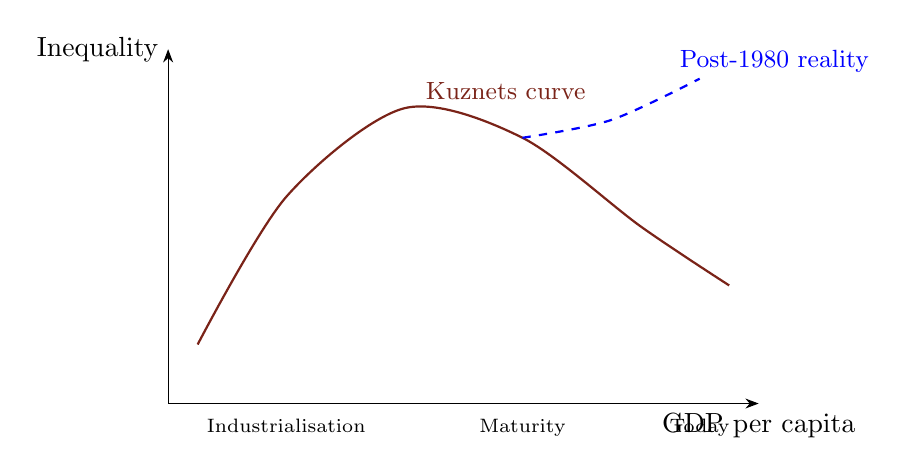
\begin{tikzpicture}[scale=0.75, >=Stealth]
  % Axes
  \draw[->] (0,0) -- (10,0) node[below] {GDP per capita};
  \draw[->] (0,0) -- (0,6) node[left] {Inequality};
  % Kuznets inverted-U
  \draw[thick, UoERed] plot[smooth] coordinates
    {(0.5,1) (2,3.5) (4,5) (6,4.5) (8,3) (9.5,2)};
  \node[right, font=\small, UoERed] at (4.2, 5.3) {Kuznets curve};
  % Piketty's amendment
  \draw[thick, dashed, blue] plot[smooth] coordinates
    {(6,4.5) (7.5,4.8) (9,5.5)};
  \node[right, font=\small, blue] at (8.5, 5.8) {Post-1980 reality};
  % Labels
  \node[below, font=\scriptsize] at (2, -0.1) {Industrialisation};
  \node[below, font=\scriptsize] at (6, -0.1) {Maturity};
  \node[below, font=\scriptsize] at (9, -0.1) {Today};
\end{tikzpicture}
\end{center}
\vspace{0.3em}
Kuznets (1955) predicted the inverted U. Piketty showed inequality
can \textbf{rise again} --- the natural tendency of capitalism when $r > g$.
\end{frame}

\begin{frame}{Piketty's Central Formula: $r > g$}
\begin{columns}[T]
\column{0.55\textwidth}
\begin{block}{The Inequality}
\[
  r > g
\]
\begin{itemize}
  \item $r$ = rate of return on capital (dividends, interest, rents,
        capital gains)
  \item $g$ = growth rate of the economy (GDP growth)
\end{itemize}
\end{block}
\vspace{0.5em}
When $r > g$: inherited wealth grows \textbf{faster} than earned income.
The rich get richer, not through effort, but through the \textit{mathematics
of compound returns}.
\column{0.4\textwidth}
\begin{block}{Historical Values}
\begin{center}
\begin{tabular}{lcc}
\toprule
Era & $r$ & $g$ \\
\midrule
1870--1914 & 5\% & 1.5\% \\
1914--1950 & 1\% & 1.5\% \\
1950--2012 & 5\% & 3.5\% \\
2012--2100? & 4\% & 1.5\% \\
\bottomrule
\end{tabular}
\end{center}
\end{block}
\end{columns}
\end{frame}

\begin{frame}{Aiyagari (1994): Inequality from Identical People}
\begin{columns}[T]
\column{0.55\textwidth}
\begin{itemize}
  \item Can we explain inequality \textit{without} assuming people
        are fundamentally different?
  \item \textbf{S.\ Rao Aiyagari} (1994): yes.
  \item All agents are \textit{identical} --- same preferences,
        abilities, initial conditions.
  \item The only difference is \alert{luck}: random income shocks
        modelled as a Markov chain.
  \item The wealth distribution that emerges is highly unequal
        and right-skewed.
\end{itemize}
\column{0.4\textwidth}
\begin{block}{Key Insight}
\textbf{Inequality is an emergent property} of an economy with
incomplete markets and idiosyncratic risk --- not necessarily the
result of differences in talent, effort, or inheritance.
\end{block}
\end{columns}
\end{frame}

\begin{frame}{Edinburgh Connection: Angus Deaton}
\begin{columns}[T]
\column{0.55\textwidth}
\begin{itemize}
  \item \textbf{Angus Deaton} (1945--2025), born in Edinburgh, educated
        at Fettes College.
  \item Nobel Prize in Economics, 2015.
  \item His book \textit{The Great Escape} (2013): humanity has made
        extraordinary progress, but it has been \textbf{deeply uneven}.
  \item Developed household survey methods and consumption-based
        measures that let economists \textit{see} inequality where
        GDP averages hid it.
\end{itemize}
\column{0.4\textwidth}
\begin{block}{Scottish Roots}
The same empirical rigour and moral seriousness that characterised
the Scottish Enlightenment --- the insistence that economics must
grapple with real data about real lives, not just elegant abstractions.
\end{block}
\end{columns}
\end{frame}

\begin{frame}{From History to Computation}
\begin{center}
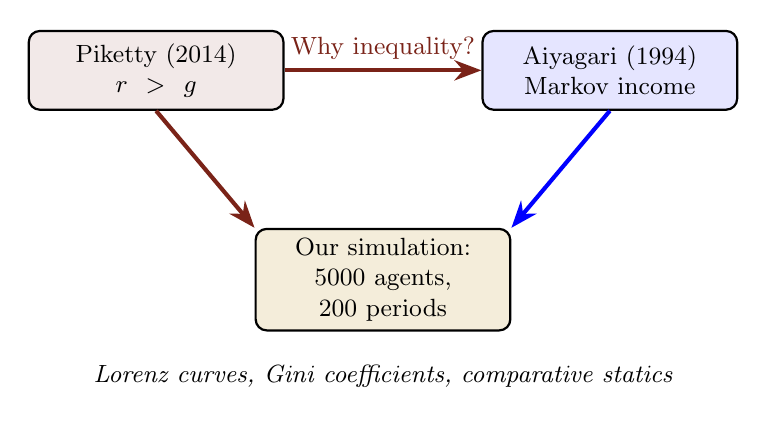
\begin{tikzpicture}[>=Stealth, thick, scale=0.85,
  box/.style={draw, rounded corners, minimum width=3.2cm, minimum height=1cm,
              font=\small, text width=3cm, align=center}]
  \node[box, fill=UoERed!10] (piketty) {Piketty (2014)\\$r > g$};
  \node[box, fill=blue!10, right=2.5cm of piketty] (aiyagari)
    {Aiyagari (1994)\\Markov income};
  \node[box, fill=UoEGold!15, below=2cm of $(piketty)!0.5!(aiyagari)$] (sim)
    {Our simulation:\\5000 agents,\\200 periods};
  \draw[->, line width=1.5pt, UoERed] (piketty) -- node[above, font=\small]
    {Why inequality?} (aiyagari);
  \draw[->, line width=1.5pt, UoERed] (piketty.south) -- (sim.north west);
  \draw[->, line width=1.5pt, blue] (aiyagari.south) -- (sim.north east);
  \node[below=0.3cm of sim, font=\small\itshape] {Lorenz curves, Gini coefficients,
    comparative statics};
\end{tikzpicture}
\end{center}
\end{frame}

% -------------------------------------------------------------
\section{Part II --- The Computation}
% -------------------------------------------------------------

\begin{frame}[fragile]{Setting Up}
\begin{lstlisting}
import numpy as np
import matplotlib.pyplot as plt

np.random.seed(42)  # for reproducibility
\end{lstlisting}
\vspace{0.5em}
\begin{itemize}
  \item \texttt{numpy} --- numerical arrays, random number generation,
        linear algebra
  \item \texttt{matplotlib} --- plotting distributions and Lorenz curves
  \item No optimisation library needed this week --- the model is
        \textbf{simulated}, not solved analytically
\end{itemize}
\end{frame}

\begin{frame}{Income as a Markov Chain}
Each agent's income follows a \textbf{Markov chain} --- next period's
income depends \textit{only} on this period's income.
\vspace{0.5em}
\begin{columns}[T]
\column{0.45\textwidth}
\begin{center}
\begin{tabular}{lcc}
\toprule
State & Label & Income $y$ \\
\midrule
0 & Low    & 0.5 \\
1 & Medium & 1.0 \\
2 & High   & 2.0 \\
\bottomrule
\end{tabular}
\end{center}
\column{0.5\textwidth}
The \textbf{transition matrix} $P$:
\[
P = \begin{pmatrix}
0.6 & 0.3 & 0.1 \\
0.2 & 0.6 & 0.2 \\
0.1 & 0.3 & 0.6
\end{pmatrix}
\]
Entry $P_{ij}$ = probability of moving from state $i$ to state $j$.
Each row sums to 1.
\end{columns}
\end{frame}

\begin{frame}{The Markov Chain: Transitions}
\begin{center}
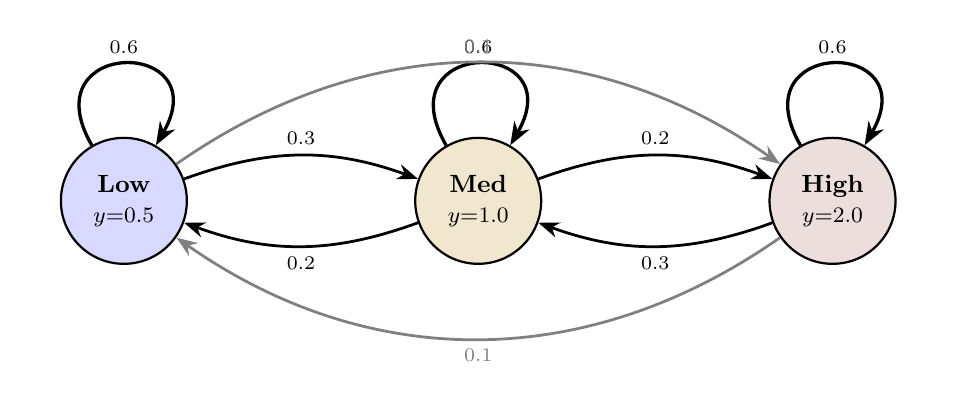
\begin{tikzpicture}[>=Stealth, thick, scale=0.9,
  mcstate/.style={draw, circle, minimum size=1.6cm, font=\small\bfseries,
                  align=center}]
  \node[mcstate, fill=blue!15] (L) at (0,0) {Low\\ \footnotesize$y{=}0.5$};
  \node[mcstate, fill=UoEGold!20] (M) at (5,0) {Med\\ \footnotesize$y{=}1.0$};
  \node[mcstate, fill=UoERed!15] (H) at (10,0) {High\\ \footnotesize$y{=}2.0$};
  % Self-loops
  \draw[->, line width=1.2pt] (L) to[out=120, in=60, looseness=5] node[above, font=\scriptsize] {0.6} (L);
  \draw[->, line width=1.2pt] (M) to[out=120, in=60, looseness=5] node[above, font=\scriptsize] {0.6} (M);
  \draw[->, line width=1.2pt] (H) to[out=120, in=60, looseness=5] node[above, font=\scriptsize] {0.6} (H);
  % L <-> M
  \draw[->, line width=1pt] (L) to[bend left=20] node[above, font=\scriptsize] {0.3} (M);
  \draw[->, line width=1pt] (M) to[bend left=20] node[below, font=\scriptsize] {0.2} (L);
  % M <-> H
  \draw[->, line width=1pt] (M) to[bend left=20] node[above, font=\scriptsize] {0.2} (H);
  \draw[->, line width=1pt] (H) to[bend left=20] node[below, font=\scriptsize] {0.3} (M);
  % L <-> H
  \draw[->, line width=1pt, gray] (L) to[bend left=35] node[above, font=\scriptsize] {0.1} (H);
  \draw[->, line width=1pt, gray] (H) to[bend left=35] node[below, font=\scriptsize] {0.1} (L);
\end{tikzpicture}
\end{center}
\vspace{0.5em}
Moderate persistence: agents \textit{tend} to stay in their current state
but can move up or down. A low-income agent has a 60\% chance of staying
low, 30\% of rising to medium, 10\% of jumping to high.
\end{frame}

\begin{frame}[fragile]{Transition Matrix in Python}
\begin{lstlisting}
# Income levels for three states
income_levels = np.array([0.5, 1.0, 2.0])

# Transition matrix: P[i,j] = Prob(state j | state i)
P = np.array([
    [0.6, 0.3, 0.1],  # from Low
    [0.2, 0.6, 0.2],  # from Medium
    [0.1, 0.3, 0.6],  # from High
])

print("Row sums:", P.sum(axis=1))  # [1. 1. 1.]
\end{lstlisting}
\vspace{0.5em}
Key properties of any transition matrix:
\begin{itemize}
  \item All entries $\geq 0$ (probabilities)
  \item Each row sums to 1 (must go \textit{somewhere})
  \item Diagonal entries = \textbf{persistence}
\end{itemize}
\end{frame}

\begin{frame}{The Stationary Distribution}
A Markov chain has a \textbf{stationary distribution} $\pi$ such that
$\pi P = \pi$.
\vspace{0.3em}
\begin{itemize}
  \item $\pi$ tells us the long-run fraction of the population in each state.
  \item Found by computing the left eigenvector of $P$ with eigenvalue 1.
\end{itemize}
\vspace{0.5em}
For our transition matrix:
\[
\pi = \bigl(\pi_{\text{Low}},\; \pi_{\text{Med}},\; \pi_{\text{High}}\bigr)
    \approx (0.235,\; 0.412,\; 0.353)
\]
\vspace{0.3em}
Long-run mean income:
$\bar{y} = 0.235 \times 0.5 + 0.412 \times 1.0 + 0.353 \times 2.0 \approx 1.24$
\end{frame}

\begin{frame}[fragile]{Computing the Stationary Distribution}
\begin{lstlisting}
# Solve pi @ P = pi  <=>  left eigenvector with eigenvalue 1
eigenvalues, eigenvectors = np.linalg.eig(P.T)

idx = np.argmin(np.abs(eigenvalues - 1.0))
pi = np.real(eigenvectors[:, idx])
pi = pi / pi.sum()  # normalise

for state, prob in zip(['Low', 'Medium', 'High'], pi):
    print(f"  {state}: {prob:.4f}")

mean_income = np.dot(pi, income_levels)
print(f"Long-run mean income: {mean_income:.4f}")
\end{lstlisting}
\end{frame}

\begin{frame}[fragile]{Simulating 5000 Agents}
\begin{lstlisting}
def simulate_markov(P, n_agents, n_periods, seed=42):
    rng = np.random.default_rng(seed)
    n_states = P.shape[0]
    states = np.zeros((n_agents, n_periods), dtype=int)
    states[:, 0] = rng.choice(n_states, size=n_agents, p=pi)
    for t in range(1, n_periods):
        u = rng.random(n_agents)
        for s in range(n_states):
            mask = (states[:, t-1] == s)
            cum_probs = np.cumsum(P[s])
            states[mask, t] = np.searchsorted(cum_probs, u[mask])
    return states

n_agents, n_periods = 5000, 200
state_paths = simulate_markov(P, n_agents, n_periods)
income_paths = income_levels[state_paths]
\end{lstlisting}
Each agent follows the same Markov chain --- the only difference is \alert{luck}.
\end{frame}

\begin{frame}{From Income to Wealth: The Accumulation Equation}
Agents accumulate wealth according to:
\[
  w_{t+1} = (1 + r) \cdot w_t + y_t - c_t
\]
\begin{itemize}
  \item $w_t$ = wealth at time $t$
  \item $r$ = interest rate (return on savings)
  \item $y_t$ = income (from the Markov chain)
  \item $c_t$ = consumption
\end{itemize}
\vspace{0.5em}
\textbf{Consumption rule:} agents consume a fixed fraction $\alpha$ of resources:
\[
  c_t = \alpha \cdot \bigl((1+r) \cdot w_t + y_t\bigr), \qquad \alpha \in (0,1)
\]
\textbf{Borrowing constraint:} $w_t \geq 0$ --- agents cannot go into debt.\\[4pt]
This friction is the key to the Aiyagari model: agents \textit{cannot perfectly
insure} against bad income shocks.
\end{frame}

\begin{frame}[fragile]{Wealth Simulation in Python}
\begin{lstlisting}
def simulate_wealth(income_paths, r=0.02, alpha=0.9, w0=1.0):
    n_agents, n_periods = income_paths.shape
    wealth = np.zeros((n_agents, n_periods))
    wealth[:, 0] = w0
    for t in range(n_periods - 1):
        resources = (1 + r) * wealth[:, t] + income_paths[:, t]
        consumption = alpha * resources
        wealth[:, t+1] = np.maximum(resources - consumption, 0.0)
    return wealth

r = 0.02       # 2% interest rate
alpha = 0.9    # consume 90%, save 10%
wealth = simulate_wealth(income_paths, r=r, alpha=alpha, w0=1.0)
\end{lstlisting}
\vspace{0.3em}
\begin{itemize}
  \item All agents start with the same wealth $w_0 = 1$.
  \item After 200 periods: mean $>$ median $\Rightarrow$ \alert{right-skewed} distribution.
\end{itemize}
\end{frame}

\begin{frame}{The Stationary Wealth Distribution}
\begin{center}
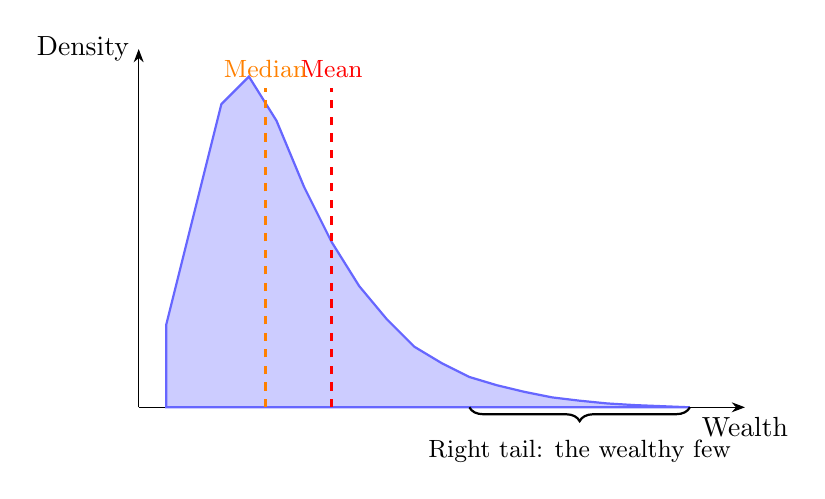
\begin{tikzpicture}[scale=0.7, >=Stealth]
  % Axes
  \draw[->] (0,0) -- (11,0) node[below] {Wealth};
  \draw[->] (0,0) -- (0,6.5) node[left] {Density};
  % Histogram-like shape: right-skewed
  \draw[thick, fill=blue!20, draw=blue!60] (0.5,0) -- (0.5,1.5) -- (1,3.5) --
    (1.5,5.5) -- (2,6) -- (2.5,5.2) -- (3,4) -- (3.5,3) -- (4,2.2) --
    (4.5,1.6) -- (5,1.1) -- (5.5,0.8) -- (6,0.55) -- (6.5,0.4) --
    (7,0.28) -- (7.5,0.18) -- (8,0.12) -- (8.5,0.07) -- (9,0.04) --
    (9.5,0.02) -- (10,0) -- cycle;
  % Mean and Median
  \draw[dashed, red, thick] (3.5,0) -- (3.5,5.8) node[above, font=\small] {Mean};
  \draw[dashed, orange, thick] (2.3,0) -- (2.3,5.8) node[above, font=\small] {Median};
  % Annotation
  \draw[decorate, decoration={brace, amplitude=5pt, mirror}, thick]
    (6,0) -- (10,0) node[midway, below=8pt, font=\small] {Right tail: the wealthy few};
\end{tikzpicture}
\end{center}
\vspace{0.3em}
Mean $>$ median: a few very wealthy agents pull the average up.\\
\textbf{Identical agents}, different luck $\Rightarrow$ \alert{unequal outcomes}.
This is Aiyagari's insight.
\end{frame}

\begin{frame}{The Lorenz Curve}
\begin{center}
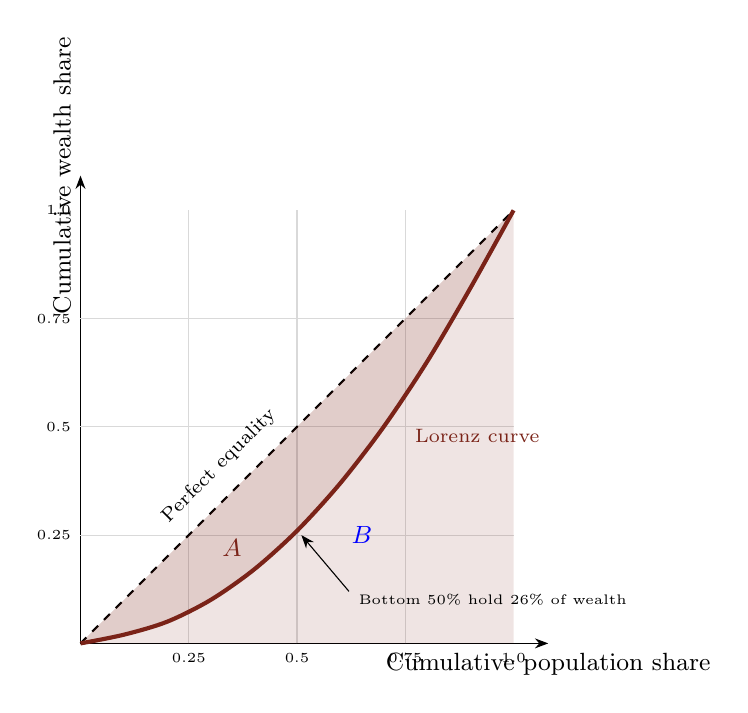
\begin{tikzpicture}[scale=5.5, >=Stealth]
  % Axes
  \draw[->] (0,0) -- (1.08,0) node[below] {\small Cumulative population share};
  \draw[->] (0,0) -- (0,1.08) node[left, rotate=90, anchor=south] {\small Cumulative wealth share};
  % Grid
  \draw[gray!30] (0.25,0) -- (0.25,1);
  \draw[gray!30] (0.5,0) -- (0.5,1);
  \draw[gray!30] (0.75,0) -- (0.75,1);
  \draw[gray!30] (0,0.25) -- (1,0.25);
  \draw[gray!30] (0,0.5) -- (1,0.5);
  \draw[gray!30] (0,0.75) -- (1,0.75);
  % Tick labels
  \foreach \x in {0.25, 0.5, 0.75, 1.0}
    \node[below, font=\tiny] at (\x, 0) {\x};
  \foreach \y in {0.25, 0.5, 0.75, 1.0}
    \node[left, font=\tiny] at (0, \y) {\y};
  % Line of equality
  \draw[black, dashed, thick] (0,0) -- (1,1);
  \node[above, font=\scriptsize, rotate=45] at (0.35, 0.38) {Perfect equality};
  % Lorenz curve (typical right-skewed distribution)
  \draw[UoERed, line width=1.5pt] plot[smooth] coordinates
    {(0,0) (0.1,0.02) (0.2,0.05) (0.3,0.10) (0.4,0.17)
     (0.5,0.26) (0.6,0.37) (0.7,0.50) (0.8,0.65)
     (0.9,0.82) (1.0,1.0)};
  \node[right, font=\scriptsize, UoERed] at (0.75, 0.48) {Lorenz curve};
  % Shaded area A
  \fill[UoERed, opacity=0.12] plot[smooth] coordinates
    {(0,0) (0.1,0.02) (0.2,0.05) (0.3,0.10) (0.4,0.17)
     (0.5,0.26) (0.6,0.37) (0.7,0.50) (0.8,0.65)
     (0.9,0.82) (1.0,1.0)} -- (0,0) -- cycle;
  \fill[UoERed, opacity=0.12] (0,0) -- (1,1) -- (1,0) -- cycle;
  % Label A
  \node[font=\small, UoERed] at (0.35, 0.22) {$A$};
  % Label B
  \node[font=\small, blue] at (0.65, 0.25) {$B$};
  % Annotation for (0.5, 0.26)
  \draw[->, thin] (0.62,0.12) -- (0.51,0.25);
  \node[right, font=\tiny] at (0.62,0.10) {Bottom 50\% hold 26\% of wealth};
\end{tikzpicture}
\end{center}
\vspace{0.2em}
$G = \dfrac{A}{A+B} = 1 - 2\displaystyle\int_0^1 L(p)\,dp$
\quad ($G=0$: perfect equality; $G=1$: perfect inequality)
\end{frame}

\begin{frame}[fragile]{Computing the Lorenz Curve}
\begin{lstlisting}
def lorenz_curve(wealth_array):
    sorted_wealth = np.sort(wealth_array)
    n = len(sorted_wealth)
    cumulative_wealth = np.cumsum(sorted_wealth)
    total_wealth = sorted_wealth.sum()
    # Prepend zero for the origin
    pop_share = np.concatenate(([0], np.arange(1, n+1) / n))
    wealth_share = np.concatenate(
        ([0], cumulative_wealth / total_wealth))
    return pop_share, wealth_share

pop_share, wealth_share = lorenz_curve(final_wealth)
plt.plot([0,1], [0,1], 'k--', label='Perfect equality')
plt.plot(pop_share, wealth_share, label='Lorenz curve')
plt.fill_between(pop_share, wealth_share, pop_share,
                 alpha=0.15)
\end{lstlisting}
\end{frame}

\begin{frame}{The Gini Coefficient}
\begin{columns}[T]
\column{0.5\textwidth}
\begin{block}{Formula}
\[
  G = 1 - 2 \int_0^1 L(p)\,dp
\]
\end{block}
\vspace{0.3em}
\begin{itemize}
  \item $G = 0$: everyone has the same wealth
  \item $G = 1$: one person has everything
\end{itemize}
\column{0.45\textwidth}
\begin{block}{Real-World Wealth Gini}
\begin{center}
\begin{tabular}{lc}
\toprule
Country & Gini \\
\midrule
Sweden       & $\approx 0.50$ \\
Germany      & $\approx 0.67$ \\
UK           & $\approx 0.73$ \\
United States & $\approx 0.85$ \\
\bottomrule
\end{tabular}
\end{center}
\end{block}
\end{columns}
\vspace{0.5em}
Wealth Gini coefficients are much higher than income Gini coefficients ---
wealth accumulates over a lifetime and across generations.
\end{frame}

\begin{frame}[fragile]{Computing the Gini Coefficient}
\begin{lstlisting}
def gini_coefficient(wealth_array):
    pop_share, wealth_share = lorenz_curve(wealth_array)
    # Area under Lorenz curve (trapezoidal rule)
    area_under_lorenz = np.trapz(wealth_share, pop_share)
    return 1 - 2 * area_under_lorenz

gini = gini_coefficient(final_wealth)
print(f"Simulated Gini: {gini:.4f}")
\end{lstlisting}
\vspace{0.5em}
\begin{block}{Wealth Shares (Typical Simulation Output)}
\begin{itemize}
  \item Top 1\% own $\sim$5--8\% of total wealth
  \item Top 10\% own $\sim$25--35\% of total wealth
  \item Bottom 50\% own $\sim$20--30\% of total wealth
\end{itemize}
\end{block}
\end{frame}

\begin{frame}{Comparative Statics: What Drives Inequality?}
\begin{center}
\begin{tabular}{lccc}
\toprule
Scenario & $r$ & Income range & Effect on Gini \\
\midrule
Baseline            & 0.02 & $[0.5,\; 1.0,\; 2.0]$ & --- \\
Higher interest rate & 0.05 & $[0.5,\; 1.0,\; 2.0]$ & $\uparrow$ \\
Higher volatility   & 0.02 & $[0.2,\; 1.0,\; 3.0]$ & $\uparrow$ \\
\bottomrule
\end{tabular}
\end{center}
\vspace{0.5em}
\begin{itemize}
  \item \textbf{Higher $r$}: the rich earn more on their savings
        $\Rightarrow$ Piketty's $r > g$ mechanism.
  \item \textbf{Greater income volatility}: bigger shocks, harder to
        self-insure $\Rightarrow$ wider wealth dispersion.
  \item Both push the Lorenz curve \textbf{further from the line of equality}.
\end{itemize}
\end{frame}

\begin{frame}[fragile]{Running the Comparative Statics}
\begin{lstlisting}
# Scenario 2: Higher interest rate
wealth_high_r = simulate_wealth(income_paths, r=0.05,
                                alpha=0.9, w0=1.0)
gini_high_r = gini_coefficient(wealth_high_r[:, -1])

# Scenario 3: Higher income volatility
income_levels_volatile = np.array([0.2, 1.0, 3.0])
income_paths_volatile = income_levels_volatile[state_paths]
wealth_volatile = simulate_wealth(income_paths_volatile,
                                  r=0.02, alpha=0.9, w0=1.0)
gini_volatile = gini_coefficient(wealth_volatile[:, -1])
\end{lstlisting}
\vspace{0.3em}
Plot all three Lorenz curves on one figure to visualise how parameter
changes shift the distribution.
\end{frame}

\begin{frame}{Lorenz Curves: Comparative Statics}
\begin{center}
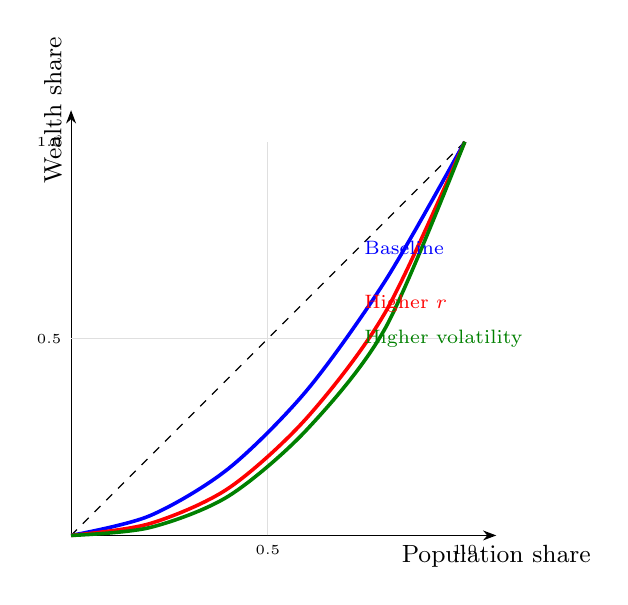
\begin{tikzpicture}[scale=5, >=Stealth]
  % Axes
  \draw[->] (0,0) -- (1.08,0) node[below] {\small Population share};
  \draw[->] (0,0) -- (0,1.08) node[left, rotate=90, anchor=south] {\small Wealth share};
  % Grid
  \draw[gray!25] (0.5,0) -- (0.5,1);
  \draw[gray!25] (0,0.5) -- (1,0.5);
  % Ticks
  \node[below, font=\tiny] at (0.5,0) {0.5};
  \node[below, font=\tiny] at (1.0,0) {1.0};
  \node[left, font=\tiny] at (0,0.5) {0.5};
  \node[left, font=\tiny] at (0,1.0) {1.0};
  % Line of equality
  \draw[black, dashed] (0,0) -- (1,1);
  % Baseline (moderate bow)
  \draw[blue, line width=1.3pt] plot[smooth] coordinates
    {(0,0) (0.2,0.05) (0.4,0.17) (0.6,0.37) (0.8,0.65) (1,1)};
  % Higher r (more bowed)
  \draw[red, line width=1.3pt] plot[smooth] coordinates
    {(0,0) (0.2,0.03) (0.4,0.12) (0.6,0.30) (0.8,0.57) (1,1)};
  % Higher volatility (most bowed)
  \draw[green!50!black, line width=1.3pt] plot[smooth] coordinates
    {(0,0) (0.2,0.02) (0.4,0.10) (0.6,0.27) (0.8,0.53) (1,1)};
  % Legend
  \node[font=\scriptsize, blue, right] at (0.72, 0.73) {Baseline};
  \node[font=\scriptsize, red, right] at (0.72, 0.59) {Higher $r$};
  \node[font=\scriptsize, green!50!black, right] at (0.72, 0.50) {Higher volatility};
\end{tikzpicture}
\end{center}
More bowed $=$ more unequal. Both higher $r$ and higher volatility
\textbf{increase} the Gini coefficient.
\end{frame}

\begin{frame}{How the Gini Evolves Over Time}
\begin{center}
\begin{tikzpicture}[scale=0.7, >=Stealth]
  % Axes
  \draw[->] (0,0) -- (10.5,0) node[below] {Period};
  \draw[->] (0,0) -- (0,6.5) node[left] {Gini};
  % Tick labels
  \node[below, font=\scriptsize] at (0,0) {0};
  \node[below, font=\scriptsize] at (2.5,0) {50};
  \node[below, font=\scriptsize] at (5,0) {100};
  \node[below, font=\scriptsize] at (7.5,0) {150};
  \node[below, font=\scriptsize] at (10,0) {200};
  \node[left, font=\scriptsize] at (0,0) {0};
  \node[left, font=\scriptsize] at (0,5) {$G^*$};
  % Gini path: starts near 0, rises, converges
  \draw[thick, blue] plot[smooth] coordinates
    {(0,0.2) (0.5,1.5) (1,2.5) (1.5,3.2) (2,3.7) (2.5,4.0)
     (3,4.2) (4,4.5) (5,4.7) (6,4.8) (7,4.85) (8,4.9) (9,4.92) (10,4.93)};
  % Converged value
  \draw[dashed, red] (0,4.93) -- (10,4.93);
  \node[right, font=\small, red] at (10,5.2) {Steady state};
\end{tikzpicture}
\end{center}
\vspace{0.3em}
All agents start with $w_0 = 1$ (Gini $\approx 0$). As idiosyncratic shocks
accumulate, inequality rises and \textbf{converges to a steady state}.\\[4pt]
Inequality is \alert{endogenous} --- emerging from luck alone.
\end{frame}

% -------------------------------------------------------------
\section{Part III --- Exercises \& Discussion}
% -------------------------------------------------------------

\begin{frame}{Exercise 1: Income Mobility and Persistence}
The transition matrix $P$ determines how \textit{persistent} income shocks are.
\vspace{0.5em}
\begin{enumerate}
  \item[(a)] Create a \textbf{high-persistence} transition matrix
    (diagonal = 0.8, off-diagonals split equally). Simulate 5000 agents
    for 200 periods. Compute the Gini.
  \item[(b)] Create a \textbf{low-persistence} matrix (diagonal = 0.4).
    Simulate and compute the Gini.
  \item[(c)] Plot the Lorenz curves for high-persistence, low-persistence,
    and baseline on a single figure. Which is most unequal? Why?
  \item[(d)] Plot Gini vs.\ persistence for diagonal values
    $\{0.3, 0.4, 0.5, 0.6, 0.7, 0.8, 0.9\}$.
\end{enumerate}
\vspace{0.5em}
\begin{alertblock}{Intuition}
Higher persistence $\Rightarrow$ long runs of bad (or good) luck
$\Rightarrow$ larger wealth differences $\Rightarrow$ \textbf{more inequality}.
\end{alertblock}
\end{frame}

\begin{frame}{Exercise 2: Progressive Taxation}
Implement a progressive tax-and-transfer system:
\[
\text{tax}(y) = \begin{cases}
0.1 \cdot y & \text{if } y \leq 1.0 \\[3pt]
0.1 + 0.4 \cdot (y - 1.0) & \text{if } y > 1.0
\end{cases}
\]
\vspace{0.3em}
\begin{enumerate}
  \item[(a)] Compute total tax revenue per period; redistribute equally
    as a lump-sum transfer. Simulate with post-tax income
    $y_t^{\text{net}} = y_t - \text{tax}(y_t) + \text{transfer}$.
  \item[(b)] Compare Gini with and without taxation.
    Plot both Lorenz curves.
  \item[(c)] Raise the top rate from 0.4 to 0.6. How much further
    does the Gini fall? Diminishing returns?
  \item[(d)] Plot wealth distributions for no-tax, moderate-tax,
    and high-tax. Discuss the equality--efficiency trade-off.
\end{enumerate}
\end{frame}

\begin{frame}{Exercise 3: Piketty's $r > g$}
\begin{enumerate}
  \item[(a)] Add economic growth: $y_t = y_0 \cdot (1+g)^t$.
    Simulate with $r = 0.04$, $g = 0.02$ ($r > g$).
    Track the Gini over 500 periods.
  \item[(b)] Simulate with $r = 0.02$, $g = 0.04$ ($r < g$).
    Compare the two Gini trajectories on one plot.
  \item[(c)] For the $r > g$ case, compute the top 10\% wealth share
    over time. Does it stabilise or keep growing?
  \item[(d)] Simulate Piketty's historical narrative:
    \begin{itemize}
      \item Periods 1--200: $r > g$ (Gilded Age)
      \item Periods 200--350: $r < g$ (Great Compression)
      \item Periods 350--500: $r > g$ (Great Divergence)
    \end{itemize}
    Plot the Gini over all 500 periods. Does it resemble the
    historical \textbf{U-shape} of inequality?
\end{enumerate}
\end{frame}

% -------------------------------------------------------------
\section{Quiz}
% -------------------------------------------------------------

\begin{frame}{Quiz: Conceptual Questions (1/2)}
\textbf{Q1.} Piketty's $r > g$ means that when $r$ exceeds $g$: \\[3pt]
\quad (a) The economy enters recession \quad
(b) \alert{Inherited wealth outpaces earned income} \\
\quad (c) Inflation accelerates \quad
(d) Government debt becomes unsustainable
\vspace{0.8em}

\textbf{Q2.} A Gini coefficient of 0 means: \\[3pt]
\quad (a) Everyone has zero wealth \quad
(b) One person has all the wealth \\
\quad (c) \alert{Wealth is perfectly equally distributed} \quad
(d) The economy is in autarky
\vspace{0.8em}

\textbf{Q3.} The Lorenz curve plots: \\[3pt]
\quad (a) Income over time \quad
(b) \alert{Cumulative wealth share vs.\ cumulative population share} \\
\quad (c) GDP growth vs.\ inflation \quad
(d) Supply against demand
\end{frame}

\begin{frame}{Quiz: Conceptual Questions (2/2)}
\textbf{Q4.} In the Aiyagari model, inequality arises because: \\[3pt]
\quad (a) Agents have different preferences \\
\quad (b) Some agents are inherently smarter \\
\quad (c) \alert{Identical agents face uninsurable idiosyncratic shocks} \\
\quad (d) The government redistributes from poor to rich
\vspace{0.8em}

\textbf{Q5.} Piketty argued that the mid-20th-century decline in inequality was: \\[3pt]
\quad (a) The natural tendency of capitalism \\
\quad (b) \alert{An anomaly caused by wars, depression, and progressive taxation} \\
\quad (c) The result of superior economic theory \\
\quad (d) A statistical illusion
\end{frame}

\begin{frame}{Quiz: Computational Questions (1/2)}
\textbf{Q6.} If the Lorenz curve passes through $(0.5,\; 0.2)$: \\[3pt]
\quad (a) \alert{The poorest 50\% hold 20\% of total wealth} \\
\quad (b) The richest 20\% hold 50\% \quad
(c) Average wealth is 0.2 \quad
(d) $G = 0.5$
\vspace{0.8em}

\textbf{Q7.} A Gini of 0.85 (US wealth) indicates: \\[3pt]
\quad (a) Moderate inequality \quad
(b) Near-perfect equality \\
\quad (c) \alert{Very high inequality --- Lorenz curve bows far below equality} \\
\quad (d) 85\% of people have equal wealth
\vspace{0.8em}

\textbf{Q8.} The stationary distribution $\pi$ of a Markov chain satisfies: \\[3pt]
\quad (a) $\pi = P$ \quad
(b) \alert{$\pi P = \pi$} \quad
(c) $\pi + P = 1$ \quad
(d) $\pi P = 0$
\end{frame}

\begin{frame}{Quiz: Computational Questions (2/2)}
\textbf{Q9.} Increasing the persistence of the income Markov chain will: \\[3pt]
\quad (a) Decrease inequality (more stable income) \\
\quad (b) \alert{Increase inequality (long runs of bad/good luck)} \\
\quad (c) Have no effect \quad
(d) Make $G = 1$
\vspace{0.8em}

\textbf{Q10.} The borrowing constraint $w_t \geq 0$ matters because: \\[3pt]
\quad (a) It prevents agents from saving \\
\quad (b) It ensures all agents have the same wealth \\
\quad (c) \alert{It prevents perfect insurance, generating inequality} \\
\quad (d) It makes the interest rate irrelevant
\end{frame}

% -------------------------------------------------------------
\section{Key Takeaways}
% -------------------------------------------------------------

\begin{frame}{What We Learned This Week}
\begin{enumerate}
  \item \textbf{Piketty} (2014) showed that rising inequality is the
        historical norm; the mid-20th-century compression was the exception.
  \item The formula $r > g$ captures the tendency for capital returns to
        outpace growth, concentrating wealth.
  \item \textbf{Aiyagari} (1994) demonstrated that inequality can emerge
        from \textit{identical} agents facing idiosyncratic shocks ---
        inequality as an \alert{emergent property}.
  \item \textbf{Markov chains} model persistent income processes;
        Monte Carlo simulation generates wealth distributions.
  \item The \textbf{Lorenz curve} and \textbf{Gini coefficient} are
        the standard tools for measuring inequality.
  \item \textbf{Comparative statics}: higher $r$ and greater income
        volatility both increase inequality.
\end{enumerate}
\end{frame}

\begin{frame}{Further Reading}
\begin{itemize}
  \item Piketty, T.\ \textit{Capital in the Twenty-First Century} (2014),
        Introduction and Chs.~1, 7--12.
  \item Aiyagari, S.R.\ ``Uninsured Idiosyncratic Risk and Aggregate Saving,''
        \textit{QJE} (1994).
  \item Deaton, A.\ \textit{The Great Escape: Health, Wealth, and the Origins
        of Inequality} (2013).
  \item Piketty, T.\ and Saez, E.\ ``Income Inequality in the United States,
        1913--1998,'' \textit{QJE} (2003).
  \item Kuznets, S.\ ``Economic Growth and Income Inequality,''
        \textit{AER} (1955).
\end{itemize}
\vspace{1em}
\begin{center}
\textbf{Next week:} from the distribution of wealth \textit{within} countries
to the dynamics of growth \textit{between} them ---\\
convergence, divergence, and the puzzle of why some nations are rich
and others poor.
\end{center}
\end{frame}

\end{document}
